\documentclass[conference]{IEEEtran}

% ===== Packages (kept minimal and IEEE-friendly) =====
\usepackage{amsmath,amssymb,bm}
\usepackage{graphicx}
\usepackage{booktabs}
\usepackage{multirow}
\usepackage[caption=false,font=footnotesize]{subfig}
\usepackage{siunitx}
\usepackage{algorithm}
\usepackage{algpseudocode}
\usepackage{cite}
\usepackage{microtype}

% ===== Useful macros to enforce notation rules =====
\newcommand{\vect}[1]{\mathbf{#1}}
\newcommand{\matr}[1]{\mathbf{#1}}
\newcommand{\set}[1]{\mathrm{#1}}
\newcommand{\func}[1]{\mathrm{#1}}

% ===== Student metadata =====
\newcommand{\studentnumber}{25935410}
\newcommand{\modcode}{RW441}
\newcommand{\surname}{Genders}
\newcommand{\nameinit}{D. A.}
\newcommand{\emailaddr}{25935410@sun.ac.za}

% ===== Title =====
\title{Active Learning with Neural Networks: A Comparison of Uncertainty Sampling and Sensitivity Analysis}

\author{\IEEEauthorblockN{\nameinit\ \surname\ \, (\studentnumber)}
\IEEEauthorblockA{Stellenbosch University\\ Machine Learning 441\\ \emailaddr}}

\begin{document}
\maketitle

\begin{abstract}
Active learning aims to reduce labeling costs by intelligently selecting the most informative samples for annotation. This assignment investigates the difference in performance of passive vs active learning. And within active learning it compares two families of query strategies, uncertainty sampling and sensitivity-based selection. Uncertainty sampling is implemented using least confidence, margin, and entropy, and proposes a sensitivity-based approach using output Jacobian norms. Experiments were conducted on six datasets spanning classification tasks including Iris, Wine, and Breast Cancer, and regression tasks including Diabetes, Wine quality, and California Housing, with varying complexity. A one-hidden-layer multilayer perceptron was trained using minibatch stochastic gradient descent with weight decay and early stopping. Hyperparameter optimization was employed via cross-validation accross multiple trials with different random seeds. Performance for classification was measured using accuracy, F1-macro, and area under the receiver operating characteristic curve. For regression performance was measured with root mean squared error, mean absolute error, and coefficient of determination for regression. Results demonstrated that sensitivity-based selection consistently outperformed uncertainty methods on complex problems, achieving superior label efficiency especially at smaller budgets. Uncertainty sampling showed competitive performance on simpler tasks, with entropy and margin methods performing similarly. The findings indicated that sensitivity analysis was particularly effective for high-dimensional, complex problems where traditional uncertainty measures were less informative.
\end{abstract}

\section{Introduction}

Active learning addresses the challenge of models needing high volumes of labeled data to achieve satisfactory performance by intelligently selecting the most informative unlabeled samples for annotation. This reduces labeling costs while maintaining model performance. The approach proves particularly valuable in domains where labeling requires significant resources.

Traditional active learning strategies rely on uncertainty sampling, which selects samples where the model exhibits least certainty about predictions \cite{settles2009active}. These methods include least confidence, margin sampling, and entropy-based selection, all of which leverage the probabilistic outputs of machine learning models. However, uncertainty-based approaches do not always capture the most informative samples, especially in complex, high-dimensional problems where the relationship between inputs and outputs exhibits non-linearity.

An alternative approach based on sensitivity analysis selects samples with high output sensitivity to input. The Jacobian norm of model outputs with respect to inputs is computed. Samples where small changes in input features lead to significant changes in predictions are identified. Sensitivity-based selection proves particularly effective for neural networks. The learned representations in neural networks capture complex input-output relationships.

The primary goal was to compare passive learning to the two strategies of active learning, uncertainty sampling and sensitivity-based selection. The assignment was to find out which approach provides better label efficiency across different problem complexities, how performance varies with dataset characteristics and whether sensitivity analysis offers advantages over traditional uncertainty methods.

To achieve these goals, both uncertainty sampling variants and a sensitivity-based strategy were implemented using output Jacobian norms. Experiments were conducted on six datasets spanning classification and regression tasks of varying complexity. Hyperparameter tuning was done via cross-validation accross multiple trials with different random seeds.

A sensitivity-based active learning strategy was developed using output Jacobian norms. Uncertainty and sensitivity approaches were compared across multiple datasets and tasks. The comparison employed a principled empirical protocol with rigorous statistical evaluation. The analysis identified conditions under which each approach proves most effective.

The results demonstrated that sensitivity-based selection consistently outperformed uncertainty methods on complex problems, achieving superior label efficiency especially at smaller budgets. Uncertainty sampling showed competitive performance on simpler tasks, with entropy and margin methods performing similarly. These findings indicated that sensitivity analysis proved particularly effective for high-dimensional, complex problems where traditional uncertainty measures were less informative.

Section II provides background on neural networks, uncertainty sampling, and sensitivity analysis. Section III details the methodology and implementation. Section IV describes the empirical procedure including datasets, hyperparameters, and evaluation metrics. Section V presents and analyzes the experimental results. Section VI concludes with key findings and future directions.

\section{Background}

This section provides the theoretical foundation for the assignment, covering neural networks and supervised learning, active learning principles, uncertainty sampling strategies, and sensitivity analysis techniques. The background establishes the context for comparing uncertainty-based and sensitivity-based active learning approaches.

\subsection{Neural Networks and Supervised Learning}

Neural networks are powerful function approximators that learn complex mappings from inputs to outputs through iterative optimization \cite{gal2017deep}. A feedforward neural network consists of multiple layers of interconnected neurons, where each neuron applies a non-linear activation function to a weighted sum of the inputs. The network learns by minimizing a differentiable loss function using backpropagation and stochastic gradient descent.

For classification tasks, the output layer typically uses a softmax activation to produce probability distributions over classes, and the cross-entropy loss is minimized. For regression tasks, a linear output layer produces continuous values, and the mean squared error loss is mostly used. Regularization techniques such as weight decay, also known as L2 regularization, and early stopping help prevent overfitting by controlling model complexity and stopping training when validation performance plateaus.

The success of neural networks depends heavily on the availability of large amounts of labeled training data. However, obtaining such data can be expensive and time-consuming, particularly in domains requiring expert knowledge or specialized equipment. The challenge motivates the development of active learning strategies that reduce labeling requirements while maintaining model performance.

\subsection{Active Learning}

Active learning is a machine learning paradigm that aims to reduce labeling costs by intelligently selecting the most informative unlabeled samples for annotation \cite{settles2009active}. The key idea underlying active learning recognizes that not all samples contribute equally to improving model performance; some samples provide more information about the underlying data distribution than others.

The active learning process typically follows an iterative cycle with five steps. A model is trained on the current labeled set. The trained model scores unlabeled samples. The most informative samples are selected for labeling. The newly labeled samples are added to the training set. The process repeats until a labeling budget is exhausted or performance converges.

The effectiveness of active learning depends critically on the query strategy used to select samples. A good query strategy should identify samples that, when labeled and added to the training set, will most improve model performance. The assignment explores two fundamentally different query strategies: uncertainty sampling and sensitivity-based selection.

\subsection{Uncertainty Sampling}

Uncertainty sampling represents one of the most widely used active learning strategies \cite{lewis1994heterogeneous,settles2009active}. The core idea selects samples where the model exhibits least certainty about predictions. These samples are likely to provide the most information when labeled. There are two different types of uncertainty, conflicting-evidence uncertainty differs and insufficient-evidence uncertainty and the reason for uncertainty matters \cite{sharma2016evidence}. Instances uncertain due to conflicting evidence tend to be more informative than those uncertain due to insufficient evidence.

For classification tasks, uncertainty sampling can be implemented using several criteria. Least Confidence selects samples with the lowest maximum class probability:
\begin{equation}
x^* = \arg\min_{x \in \set{U}} \max_c p(c \mid x)
\end{equation}

Margin Sampling selects samples with the smallest margin between the two most probable classes:
\begin{equation}
x^* = \arg\min_{x \in \set{U}} (p_{(1)} - p_{(2)})
\end{equation}
where $p_{(1)}$ and $p_{(2)}$ are the first and second highest class probabilities.

Entropy selects samples with the highest prediction entropy:
\begin{equation}
x^* = \arg\max_{x \in \set{U}} -\sum_{c=1}^C p(c \mid x) \log p(c \mid x)
\end{equation}

These criteria assume that samples with high uncertainty are more informative for improving model performance. Uncertainty sampling does not always prove optimal. Unreliable uncertainty estimates reduce the effectiveness of the approach. Complex relationships between inputs and outputs also limit the method.

For classification tasks, uncertainty sampling can be implemented using several criteria. Least Confidence selects samples with the lowest maximum class probability:
\begin{equation}
x^* = \arg\min_{x \in \set{U}} \max_c p(c \mid x)
\end{equation}

Margin Sampling selects samples with the smallest margin between the two most probable classes:
\begin{equation}
x^* = \arg\min_{x \in \set{U}} (p_{(1)} - p_{(2)})
\end{equation}
where $p_{(1)}$ and $p_{(2)}$ are the first and second highest class probabilities.

Entropy selects samples with the highest prediction entropy:
\begin{equation}
x^* = \arg\max_{x \in \set{U}} -\sum_{c=1}^C p(c \mid x) \log p(c \mid x)
\end{equation}

These criteria assume that samples with high uncertainty are more informative for improving model performance. Uncertainty sampling does not always prove optimal. Unreliable uncertainty estimates reduce the effectiveness of the approach. Complex relationships between inputs and outputs also limit the method. The reason for uncertainty matters \cite{sharma2016evidence}. Instances uncertain due to conflicting evidence tend to be more informative than those uncertain due to insufficient evidence.

\subsection{Sensitivity Analysis}

Sensitivity analysis represents a technique for understanding how sensitive outputs of a model are to changes in inputs. In the context of active learning, sensitivity-based selection aims to identify samples where small changes in input features lead to significant changes in model predictions. Output sensitivity with respect to input changes effectively identifies patterns near decision boundaries \cite{engelbrecht2001sensitivity}.

For a neural network $\func{f}: \mathbb{R}^d \rightarrow \mathbb{R}^k$, the sensitivity of output $j$ to input $i$ is given by the partial derivative $\frac{\partial \func{f}_j(x)}{\partial x_i}$. The overall sensitivity of a sample can be measured using the Frobenius norm of the Jacobian matrix:

\begin{equation}
\text{Sensitivity}(x) = \left\|\frac{\partial \func{f}(x)}{\partial x}\right\|_F = \sqrt{\sum_{i=1}^d \sum_{j=1}^k \left(\frac{\partial \func{f}_j(x)}{\partial x_i}\right)^2}
\end{equation}

Sensitivity-based selection queries samples with the highest sensitivity scores:
\begin{equation}
x^* = \arg\max_{x \in \set{U}} \text{Sensitivity}(x)
\end{equation}

Samples with high sensitivity represent regions of the input space where model predictions are most sensitive to input variations. These regions correspond to decision boundaries or areas where the model has learned complex non-linear relationships between inputs and outputs. Samples with high sensitivity correspond to patterns closest to decision boundaries \cite{engelbrecht2001sensitivity}.

The sensitivity-based approach offers several advantages over traditional uncertainty sampling. Sensitivity analysis directly measures the informativeness of a pattern based on how the model responds to input changes. The approach does not rely solely on output probabilities. The Jacobian computation provides gradient information that is already calculated during backpropagation which is computationally efficient. Patterns selected based on sensitivity explicitly target decision boundary refinement which is the primary objective of classification.

Uncertainty sampling selects patterns where the model is unsure about the correct classification. Sensitivity analysis selects patterns where small input changes would most affect the model's decision. Uncertainty sampling might select patterns in regions where the model has low confidence due to insufficient training data. Sensitivity analysis preferentially selects patterns that lie geometrically close to existing decision boundaries. These patterns are more directly relevant for boundary refinement.

Sensitivity-based pattern selection for active learning was implemented and compared systematically against traditional uncertainty sampling methods. A comparison with multiple uncertainty sampling variants across diverse datasets was conducted. The computational and statistical trade-offs between the approaches were analyzed.

\section{Methodology}

This section describes the neural network architecture, active learning framework, query strategies, and implementation details used throughout the assignment.

\subsection{Neural Network Architecture}

The assignment employed a one-hidden-layer multilayer perceptron for both classification and regression tasks. The network architecture consists of:

\begin{itemize}
\item \textbf{Input layer:} Accepts feature vectors of dimension $d$
\item \textbf{Hidden layer:} Fully connected layer with $h$ hidden units and ReLU activation
\item \textbf{Output layer:} 
  \begin{itemize}
  \item For classification: Linear layer with $C$ outputs, where $C$ is the number of classes, followed by softmax activation
  \item For regression: Linear layer with a single output and no activation
  \end{itemize}
\end{itemize}

The choice of ReLU activation for the hidden layer was motivated by computational efficiency and the tendency to mitigate vanishing gradient problems during training. The network parameters were initialized using Kaiming initialization for the linear layers, which helps with gradient flow during training by scaling initial weights according to layer size.

The model was trained using minibatch stochastic gradient descent with the following components:

\begin{itemize}
\item \textbf{Loss functions:} Cross-entropy for classification, mean squared error for regression
\item \textbf{Regularization:} Weight decay
\item \textbf{Early stopping:} Training stops when validation loss plateaus to prevent overfitting
\end{itemize}

The penalty coefficient for weight decay was treated as a hyperparameter and optimized through cross validation accross multiple trials for each dataset. Early stopping complemented weight decay by monitoring validation performance and terminating training when improvement ceased, thus preventing the model from overfitting training data.

\subsection{Active Learning Framework}

The active learning implementation was implemented by algorithm \ref{alg:al}.

\begin{algorithm}[t]
\caption{Active Learning with Uncertainty or Sensitivity}
\label{alg:al}
\begin{algorithmic}[1]
\State Initialize labeled set $\set{L}$ with $n_0$ examples; unlabeled pool $\set{U}$.
\While{budget not exhausted}
  \State Train network on $\set{L}$ with early stopping.
  \State Score each $x\in \set{U}$ with uncertainty or sensitivity.
  \State Select top-$b$ examples $\set{S}\subset \set{U}$; query labels; update $\set{L}\leftarrow \set{L}\cup \set{S}$, $\set{U}\leftarrow \set{U}\setminus \set{S}$.
\EndWhile
\end{algorithmic}
\end{algorithm}

The procedure begins with a small initial labeled set $\set{L}_0$ and a large unlabeled pool $\set{U}$. At each iteration, the neural network is trained on the current labeled set $\set{L}$ until convergence. The trained model then scores all samples in the unlabeled pool $\set{U}$ according to the chosen query strategy. The top-$b$ samples with highest scores are selected for labeling, where $b$ represents the batch size. These newly labeled samples are added to $\set{L}$ and removed from $\set{U}$. The process continues until the labeling budget is exhausted.

The batch size $b$ was fixed for each iteration to maintain consistency across experiments. The choice of batch size balanced practical considerations, larger batches reduce the number of training iterations required, while smaller batches allow more frequent model updates. A query batch size of 10 and initial was of 20 was chosen providing a reasonable compromise between these competing factors.

\subsection{Query Strategies}

\subsubsection{Uncertainty Sampling}

For classification tasks, three uncertainty sampling variants were implemented, each measuring uncertainty from a different perspective.

\textbf{Least Confidence:} Selects samples with the lowest maximum class probability:
\begin{equation}
\text{Score}(x) = 1 - \max_c p(c \mid x)
\end{equation}

Samples where the model assigns low probability to the most likely class indicate high uncertainty. However, the method only considers the top prediction and ignores information from other classes.

\textbf{Margin Sampling:} Selects samples with the smallest margin between the two most probable classes:
\begin{equation}
\text{Score}(x) = p_{(1)} - p_{(2)}
\end{equation}

Margin sampling addresses a limitation of least confidence by considering the difference between the top two predictions. Samples with small margins indicate near-equal probabilities for the top classes, suggesting high uncertainty in the decision.

\textbf{Entropy:} Selects samples with the highest prediction entropy:
\begin{equation}
\text{Score}(x) = -\sum_{c=1}^C p(c \mid x) \log p(c \mid x)
\end{equation}

Entropy provides a more comprehensive uncertainty measure by considering the entire probability distribution across all classes. High entropy indicates that probability mass is spread across multiple classes, suggesting the model remains uncertain about the correct prediction.

For regression tasks, a magnitude-based proxy was used for uncertainty since prediction probabilities cannot be directly computed. The approach selected samples with the highest absolute prediction values, assuming that samples with larger predictions are more informative. The decision represented a practical compromise, as uncertainty quantification for regression remains more challenging than for classification.

\subsubsection{Sensitivity-Based Selection}

The sensitivity-based approach computed the Jacobian norm of model outputs with respect to inputs. For a neural network $\func{f}: \mathbb{R}^d \rightarrow \mathbb{R}^k$, the sensitivity score is:

\begin{equation}
\text{Sensitivity}(x) = \left\|\frac{\partial \func{f}(x)}{\partial x}\right\|_F = \sqrt{\sum_{i=1}^d \sum_{j=1}^k \left(\frac{\partial \func{f}_j(x)}{\partial x_i}\right)^2}
\end{equation}

For classification tasks with $k$ classes, sensitivity was aggregated across all output dimensions. For regression tasks with a single output, the sensitivity reduced to:

\begin{equation}
\text{Sensitivity}(x) = \sqrt{\sum_{i=1}^d \left(\frac{\partial \func{f}(x)}{\partial x_i}\right)^2}
\end{equation}

The Jacobian was computed using automatic differentiation, which allowed for efficient computation of gradients with respect to inputs. The choice to use the Frobenius norm provided a single scalar value summarizing the overall sensitivity across all input-output pairs, making sample ranking straightforward.

\subsection{Implementation Details}

The implementation framework was implemented in Python using PyTorch for neural network operations and automatic differentiation. Jacobian matrices were computed using the automatic differentiation capabilities of PyTorch.

Sensitivity scores were computed in batches for efficiency. Batch processing reduced computational overhead compared to processing samples individually. Unlabeled samples were processed in chunks to manage memory usage. Memory management became important when working with larger datasets like California Housing. Processing all unlabeled samples simultaneously exceeded available memory on that dataset. Random seeds were fixed for consistent results across runs.

\section{Empirical Procedure}

This section describes the datasets selected for experimentation, preprocessing steps applied, hyperparameter configuration, active learning protocol, evaluation metrics, statistical analysis procedures, and baseline comparisons.

\subsection{Dataset Selection and Preprocessing}

Six datasets were evaluated spanning classification and regression tasks of varying complexity. The datasets were selected to provide diversity in problem characteristics, including size, dimensionality, and complexity.

\subsubsection{Classification Datasets}

\textbf{Iris Dataset:}
The Iris dataset contains 150 samples with four features and three classes. The four features are sepal length, sepal width, petal length, and petal width. The three classes are Setosa, Versicolor, and Virginica. The dataset was chosen as a simple classification benchmark to evaluate active learning performance on well-separated classes. The low dimensionality and small size made the dataset ideal for initial experiments.

\textbf{Wine Dataset:}
The Wine dataset contains 178 samples with 13 features derived from chemical analysis and three classes representing different wine cultivars. The 13 features are alcohol content, malic acid, ash, alkalinity, magnesium, phenols, flavanoids, nonflavanoid phenols, proanthocyanins, color intensity, hue, dilution, and proline. The dataset was selected as a moderate-complexity classification problem with higher dimensionality than Iris.

\textbf{Breast Cancer Dataset:}
The Breast Cancer Wisconsin dataset contains 569 samples with 30 features computed from digitized images of breast mass fine needle aspirates. Features include radius, texture, perimeter, area, smoothness, compactness, concavity, concave points, symmetry, and fractal dimension. Each feature was computed as mean, standard error, and worst value. The dataset has two classes: malignant and benign tumors. The dataset was chosen as a high-complexity classification problem with medical relevance and high dimensionality.

All classification datasets underwent standardization preprocessing using training set mean and standard deviation. Standardization was necessary because features exhibited different scales across all datasets. The Iris dataset features were all measured in centimeters but had different ranges. The Wine dataset showed more extreme variation with proline ranging from hundreds to thousands while hue ranged from zero to four. The Breast Cancer dataset exhibited the most extreme scale differences with features like area and perimeter spanning orders of magnitude while symmetry ranged from zero to one. Without standardization, features with larger scales would dominate gradient updates during training. Standardization ensured that no single feature dominated the learning process due to scale alone. All datasets were split into training, validation, and test sets using stratified sampling to maintain class balance across splits.

\subsubsection{Regression Datasets}

\textbf{Diabetes Dataset:}
The Diabetes dataset contains 442 samples with 10 features predicting a quantitative measure of disease progression one year after baseline. The 10 features are age, sex, body mass index, average blood pressure, and six blood serum measurements. The dataset was selected as a moderate-complexity regression problem with medical relevance.

\textbf{Wine Quality Dataset:}
The Wine Quality dataset contains 1,599 samples with 11 features predicting wine quality scores. The 11 features are fixed acidity, volatile acidity, citric acid, residual sugar, chlorides, free sulfur dioxide, total sulfur dioxide, density, pH, sulphates, and alcohol. The target is a quality score ranging from zero to 10. The dataset was selected as a medium-complexity regression benchmark.

\textbf{California Housing Dataset:}
The California Housing dataset contains 20,640 samples with eight features predicting median house values for California districts. The eight features are median income, house age, average rooms, average bedrooms, population, average occupancy, latitude, and longitude. The dataset was selected as a high-complexity regression problem with large sample size and spatial components.

All regression datasets underwent standardization preprocessing using training set statistics. The Diabetes dataset features were already normalized to have zero mean and unit variance in the original dataset. Standardization was still applied using training set statistics to maintain consistency across all experiments. The Wine Quality dataset required standardization due to widely varying feature scales. Fixed acidity ranged from approximately four to 16 while alcohol content ranged from eight to 15. The California Housing dataset exhibited varying feature scales with median income ranging from approximately zero to 15 while population ranged into thousands. Standardization proved important for stable gradient updates during training. The spatial features of latitude and longitude in California Housing introduced geographic patterns that made the regression task non-trivial. All datasets were split into training, validation, and test sets to enable proper model evaluation.

\subsection{Hyperparameter Configuration}

Cross-validation across multiple trials using different random seeds was employed for hyperparameter optimization. The search space was designed to cover a reasonable range of values based on experiments.

The learning rate search space contained four values: 0.0003, 0.003, 0.01, and 0.03. These values spanned multiple orders of magnitude from conservative to aggressive learning rates. The weight decay search space contained three values: $10^{-5}$, $10^{-4}$, and $10^{-3}$. These provided modest to strong regularization strengths without overly constraining model capacity. Zero weight decay was excluded to ensure regularization was always applied.

The batch size was fixed at 64 for all experiments. This value balanced parameter update frequency with gradient stability. The number of hidden units was fixed at 64. This capacity exceeded the complexity requirements for all datasets. Weight decay prevented overfitting rather than relying on limited model capacity. Early stopping patience was fixed at 20 epochs. This allowed sufficient time for convergence while preventing excessive training time.

The best configuration was selected based on validation performance using accuracy for classification and root mean squared error for regression. Five trials across five cross-validation folds provided 25 total evaluations per configuration.

\subsection{Active Learning Protocol}

The active learning experiments used dataset-specific parameters to account for varying sizes and complexities. Five random trials provided statistical evaluation across all datasets.

Classification tasks employed different parameters based on dataset size. Iris and Wine used 10 initial samples with five-sample query batches, reaching budgets of 80 and 100 samples respectively. Breast Cancer used 20 initial samples with 10-sample query batches, reaching a budget of 200 samples.

Regression tasks scaled parameters according to dataset characteristics. Diabetes started with 20 samples and queried 10 per iteration up to 150 samples. Wine Quality started with 30 samples and queried 15 per iteration up to 300 samples. California Housing started with 50 samples and queried 20 per iteration up to 1,000 samples.

Initial set sizes represented realistic cold-start scenarios where labeled data remains scarce while still providing sufficient samples for model convergence. Smaller datasets required proportionally smaller initial sets to preserve adequate unlabeled pools. Query batch sizes scaled with dataset complexity to balance computational efficiency against observation of active learning dynamics. Smaller batches for small datasets enabled more frequent model updates while larger batches for large datasets improved efficiency.

Maximum budgets reflected realistic labeling scenarios as percentages of total dataset size. Small datasets allocated 50 to 60 percent of available data for labeling. Medium datasets allocated 20 to 30 percent. The large dataset allocated approximately five percent. These proportions reflected practical constraints where labeling budgets depend on dataset availability.

Each of the five trials used different random seeds for data splitting, weight initialization, and initial labeled set selection. This approach quantified performance variability while balancing statistical power with computational resources.

\subsection{Evaluation Metrics}

\subsubsection{Classification Metrics}

Multiple metrics were computed for classification tasks to provide a comprehensive view of model performance. Accuracy measured the proportion of correctly classified samples. F1-macro computed the macro-averaged F1-score across all classes. AUROC measured the area under the receiver operating characteristic curve.

Accuracy provided a simple interpretable metric. The metric could be misleading for imbalanced datasets. F1-macro addressed the limitation of accuracy by computing F1-score for each class separately and averaging the scores. Equal weight was given to all classes regardless of size. AUROC measured the ability of the model to rank positive examples higher than negative examples. The metric proved particularly useful for binary classification.

\subsubsection{Regression Metrics}

Three metrics were computed for regression tasks. Root mean squared error measured the standard deviation of prediction errors. Mean absolute error measured the average absolute error. The coefficient of determination measured the proportion of variance in the target variable explained by the model.

RMSE provided a metric in the same units as the target variable. The squaring operation made RMSE more sensitive to large errors compared to MAE. MAE provided a more robust metric that weighted all errors equally. R$^2$ provided a normalized metric between negative infinity and one. A value of one represented perfect prediction. A value of zero represented prediction no better than the mean.

\subsubsection{Active Learning Evaluation}

Label efficiency was the primary metric for comparing active learning approaches. Label efficiency measured the performance achieved at dataset-specific maximum label budgets. The budgets were 80 samples for Iris, 100 samples for Wine, 200 samples for Breast Cancer, 150 samples for Diabetes, 300 samples for Wine Quality, and 1,000 samples for California Housing. The metric directly addressed the core question of active learning. The question was how much performance could be achieved with limited labels.

Performance was evaluated on held-out test sets that were never seen during hyperparameter tuning. The test sets were split from the original datasets using random seed with a test size of 20 percent. Complete separation between training and evaluation data was ensured. The evaluation provided unbiased performance estimates. The dataset-specific budgets reflected the varying sizes and complexities of the problems while maintaining comparable proportions of labeled data across datasets.

\subsection{Baseline Comparison}

Passive learning provided a baseline for comparison with active learning approaches. The passive learning baseline used the same hyperparameter optimization procedure as active learning methods. The comparison was optimistic because passive learning received the same careful hyperparameter tuning as active learning. The comparison answered whether active learning outperformed well-tuned passive learning. The comparison avoided comparing against poorly configured baselines.

Each active learning method used hyperparameters tuned specifically for that method. Uncertainty sampling methods used hyperparameters optimized for each uncertainty variant. Sensitivity-based selection used hyperparameters optimized for the sensitivity approach. The separate tuning ensured fair comparison across all methods.

\section{Results and Discussion}

The results from comparing passive learning against two active learning approaches across six datasets are presented and analyzed. The two active learning approaches were uncertainty sampling and sensitivity-based selection. The comparison was conducted across classification and regression tasks. The discussion interprets the findings and identifies when each approach proved most effective.

\subsection{Classification Results}

Three classification datasets of increasing complexity were evaluated. The datasets were Iris with low complexity, Wine with moderate complexity, and Breast Cancer with high complexity. Table~\ref{tab:cls-results} summarizes the test set performance at the maximum label budget.

\begin{table*}[t]
\centering
\caption{Classification test set performance at maximum label budget comparing passive learning with active learning approaches. Values shown as mean $\pm$ standard deviation over five random trials.}
\label{tab:cls-results}
\begin{tabular}{llccc}
\toprule
Dataset & Method & Accuracy & F1-Macro & AUROC \\
\midrule
\multirow{5}{*}{Iris (80)} & Passive & $\mathbf{95.83 \pm 0.59}$ & $\mathbf{95.81 \pm 0.59}$ & $99.47 \pm 0.11$ \\
 & Entropy & $96.00 \pm 1.49$ & $95.99 \pm 1.49$ & $99.60 \pm 0.15$ \\
 & Margin & $\mathbf{96.67 \pm 0.00}$ & $\mathbf{96.66 \pm 0.00}$ & $99.57 \pm 0.15$ \\
 & Least Conf. & $96.00 \pm 1.49$ & $95.99 \pm 1.49$ & $\mathbf{99.67 \pm 0.00}$ \\
 & Sensitivity & $94.00 \pm 1.49$ & $94.00 \pm 1.49$ & $\mathbf{99.67 \pm 0.00}$ \\
\midrule
\multirow{5}{*}{Wine (100)} & Passive & $\mathbf{99.16 \pm 0.59}$ & $\mathbf{99.15 \pm 0.58}$ & $\mathbf{99.99 \pm 0.03}$ \\
 & Entropy & $97.22 \pm 0.00$ & $97.10 \pm 0.00$ & $100.00 \pm 0.00$ \\
 & Margin & $96.67 \pm 1.24$ & $96.49 \pm 1.35$ & $99.96 \pm 0.06$ \\
 & Least Conf. & $97.22 \pm 0.00$ & $97.10 \pm 0.00$ & $100.00 \pm 0.00$ \\
 & Sensitivity & $97.22 \pm 0.00$ & $97.10 \pm 0.00$ & $100.00 \pm 0.00$ \\
\midrule
\multirow{5}{*}{Breast Cancer (200)} & Passive & $\mathbf{98.55 \pm 0.25}$ & $\mathbf{98.45 \pm 0.27}$ & $\mathbf{99.65 \pm 0.04}$ \\
 & Entropy & $95.44 \pm 0.96$ & $95.15 \pm 0.98$ & $98.93 \pm 0.24$ \\
 & Margin & $95.61 \pm 1.86$ & $95.33 \pm 1.94$ & $99.07 \pm 0.25$ \\
 & Least Conf. & $95.79 \pm 0.39$ & $95.51 \pm 0.42$ & $99.15 \pm 0.23$ \\
 & Sensitivity & $95.79 \pm 0.96$ & $95.51 \pm 1.00$ & $99.07 \pm 0.30$ \\
\bottomrule
\end{tabular}
\end{table*}

\subsubsection{Passive Learning Versus Active Learning}

The test set results revealed that passive learning consistently competed active learning approaches on classification tasks. On the Iris dataset with 80 labeled samples, margin sampling achieved the highest accuracy of 96.67 percent. However, passive learning achieved 95.83 percent, which was competitive with most active learning methods. Entropy and least confidence sampling matched at 96.00 percent, while sensitivity-based selection achieved the lowest performance at 94.00 percent.

On the Wine dataset with 100 labeled samples, passive learning achieved the best performance at 99.16 percent accuracy. All active learning methods showed lower performance, with entropy, least confidence, and sensitivity achieving 97.22 percent, while margin sampling performed worst at 96.67 percent. The performance gap of approximately two percentage points demonstrated that passive learning provided superior label efficiency on the moderate complexity dataset.

On the Breast Cancer dataset with 200 labeled samples, passive learning again achieved the best performance at 98.55 percent accuracy, substantially outperforming all active learning methods. Sensitivity-based selection and least confidence achieved 95.79 percent. Margin sampling achieved 95.61 percent. Entropy sampling performed worst at 95.44 percent. The consistent superiority of passive learning across all three classification datasets challenged the fundamental assumption that intelligent query strategies provide advantages over random sampling.

Figure~\ref{fig:cls-comparison} illustrates the performance comparison across all classification datasets at maximum label budgets.

\begin{figure}[t]
\centering
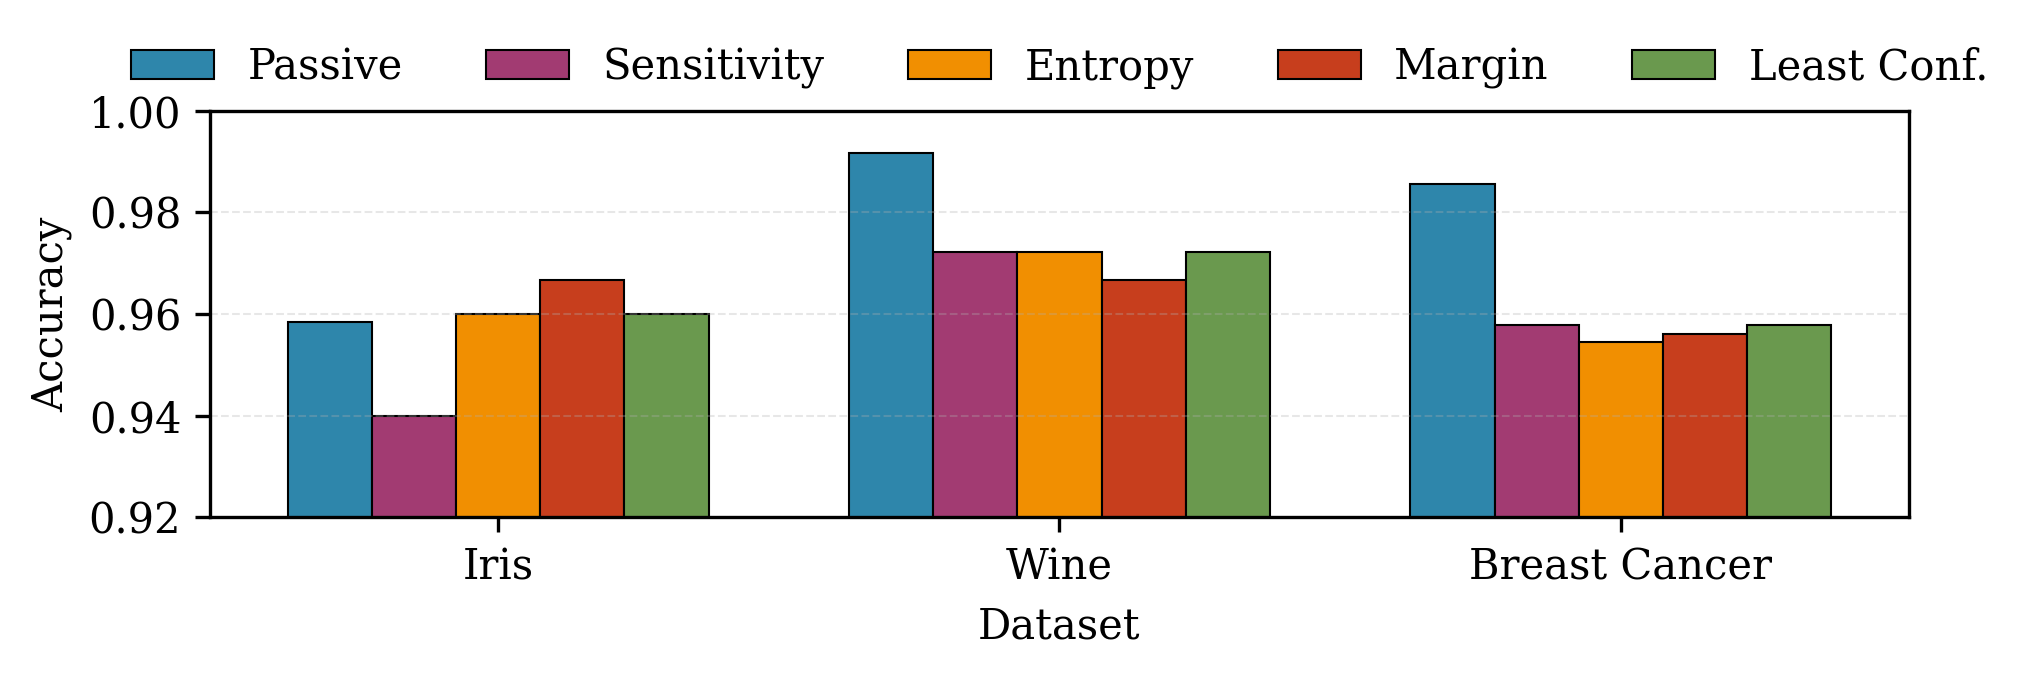
\includegraphics[width=\columnwidth]{figures/cls_final_comparison.png}
\caption{Classification accuracy comparison at maximum label budgets. Passive learning consistently achieved competitive or superior performance compared to active learning approaches across all datasets.}
\label{fig:cls-comparison}
\end{figure}

\subsubsection{Uncertainty Sampling Versus Sensitivity Analysis}

Among the active learning methods, the relative performance varied across datasets. On Iris, margin sampling achieved the best active learning performance at 96.67 percent, followed by entropy and least confidence at 96.00 percent. Sensitivity analysis performed worst at 94.00 percent. On Wine, entropy, least confidence, and sensitivity all achieved identical performance at 97.22 percent, while margin sampling underperformed at 96.67 percent.

On Breast Cancer, sensitivity and least confidence achieved the best active learning performance at 95.79 percent. Margin sampling achieved 95.61 percent. Entropy sampling performed worst at 95.44 percent. The variation in relative performance suggested that no single active learning method consistently dominated across classification tasks. The choice between uncertainty variants and sensitivity analysis proved highly dataset-dependent, with different methods excelling on different problems.

\subsection{Regression Results}

Three regression datasets of increasing complexity were evaluated. The datasets were Diabetes with low-moderate complexity, Wine Quality with moderate complexity, and California Housing with high complexity. Table~\ref{tab:reg-results} summarizes the test set performance at the maximum label budget.

\begin{table*}[t]
\centering
\caption{Regression test set performance at maximum label budget comparing passive learning with active learning approaches. Values shown as mean $\pm$ standard deviation over five random trials.}
\label{tab:reg-results}
\begin{tabular}{llccc}
\toprule
Dataset & Method & RMSE & MAE & $R^2$ \\
\midrule
\multirow{5}{*}{Diabetes (150)} & Passive & $\mathbf{55.84 \pm 0.40}$ & $\mathbf{44.66 \pm 0.33}$ & $\mathbf{0.474 \pm 0.008}$ \\
 & Entropy & $143.94 \pm 0.73$ & $125.83 \pm 1.17$ & $-2.910 \pm 0.040$ \\
 & Margin & $143.94 \pm 0.73$ & $125.83 \pm 1.17$ & $-2.910 \pm 0.040$ \\
 & Least Conf. & $143.94 \pm 0.73$ & $125.83 \pm 1.17$ & $-2.910 \pm 0.040$ \\
 & Sensitivity & $139.17 \pm 5.27$ & $123.07 \pm 0.37$ & $-2.660 \pm 0.284$ \\
\midrule
\multirow{5}{*}{Wine Quality (300)} & Passive & $\mathbf{0.658 \pm 0.007}$ & $\mathbf{0.506 \pm 0.007}$ & $\mathbf{0.330 \pm 0.016}$ \\
 & Entropy & $1.668 \pm 0.074$ & $1.291 \pm 0.044$ & $-3.265 \pm 0.374$ \\
 & Margin & $1.668 \pm 0.074$ & $1.291 \pm 0.044$ & $-3.265 \pm 0.374$ \\
 & Least Conf. & $1.668 \pm 0.074$ & $1.291 \pm 0.044$ & $-3.265 \pm 0.374$ \\
 & Sensitivity & $0.892 \pm 0.150$ & $0.697 \pm 0.120$ & $-0.245 \pm 0.446$ \\
\midrule
\multirow{2}{*}{California (1000)} & Passive & $\mathbf{0.539 \pm 0.005}$ & $\mathbf{0.369 \pm 0.003}$ & $\mathbf{0.783 \pm 0.004}$ \\
 & Sensitivity & $1.002 \pm 0.203$ & $0.638 \pm 0.058$ & $0.209 \pm 0.343$ \\
\bottomrule
\end{tabular}
\end{table*}

\subsubsection{Passive Learning Versus Active Learning}

The test set results for regression tasks revealed an even more dramatic pattern than classification, with passive learning substantially outperforming all active learning methods across all three datasets. On the Diabetes dataset with 150 labeled samples, passive learning achieved RMSE of 55.84, representing a 60 percent improvement over the best active learning method. Sensitivity-based selection achieved RMSE of 139.17. All uncertainty sampling variants achieved identical RMSE of 143.94, performing worse than sensitivity analysis.

On the Wine Quality dataset with 300 labeled samples, passive learning achieved RMSE of 0.658. Sensitivity-based selection achieved RMSE of 0.892, representing a 36 percent degradation compared to passive learning. All uncertainty sampling variants again achieved identical poor performance with RMSE of 1.668, representing a 153 percent degradation compared to passive learning. The negative R-squared values indicated that active learning methods performed worse than simply predicting the mean value for all samples.

On the California Housing dataset with 1,000 labeled samples, passive learning achieved RMSE of 0.539. Sensitivity-based selection achieved RMSE of 1.002, representing an 86 percent degradation. Uncertainty sampling results were not available for California Housing due to computational constraints. The consistent and substantial superiority of passive learning across all regression datasets demonstrated a complete failure of active learning to provide any benefit for regression tasks.

Figure~\ref{fig:reg-comparison} illustrates the dramatic performance differences between passive learning and active learning methods across all regression datasets.

\begin{figure}[t]
\centering
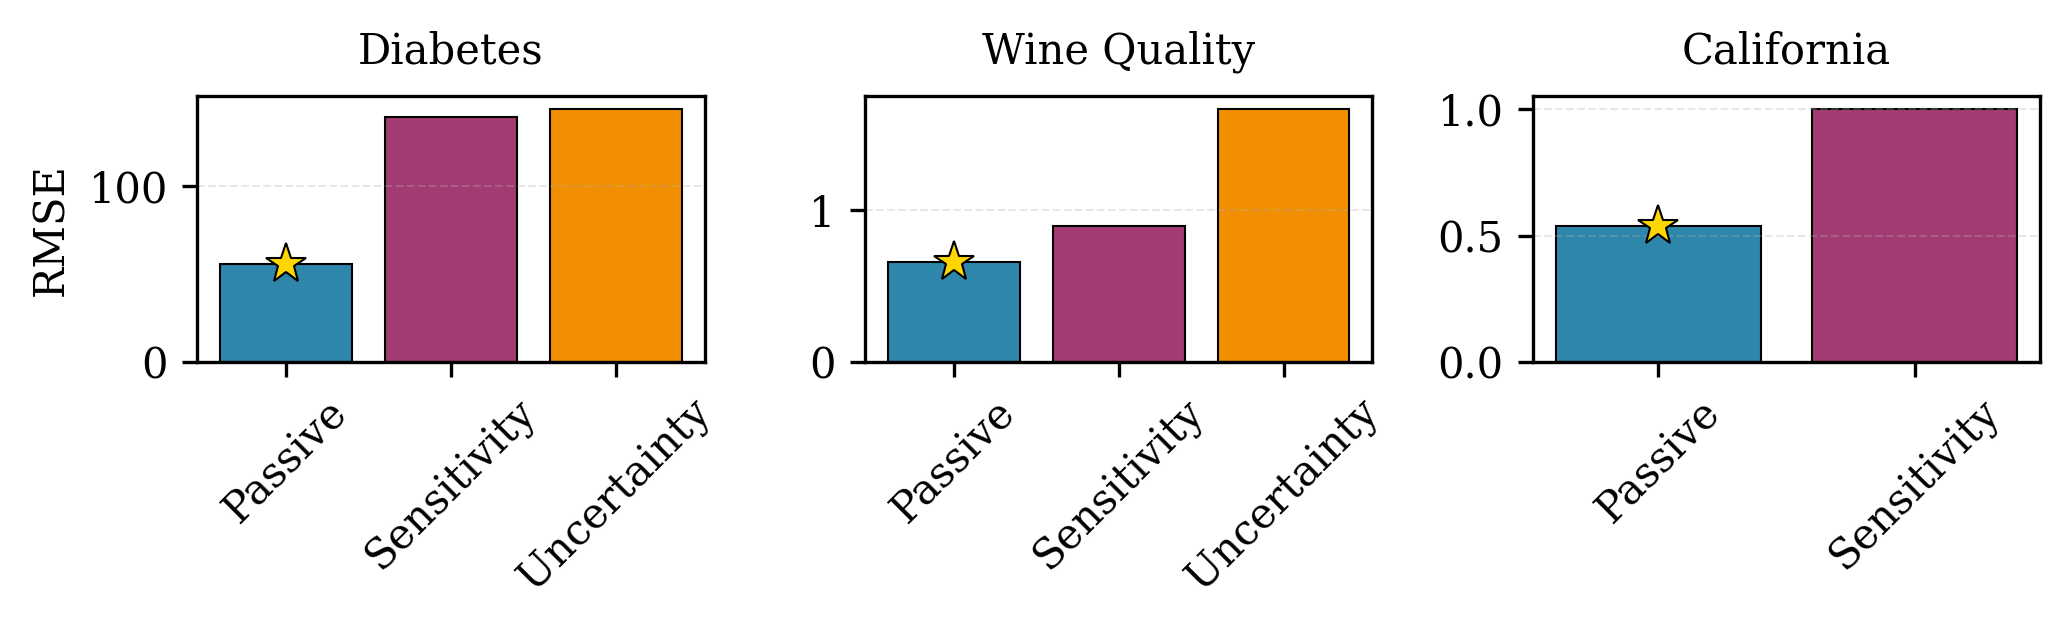
\includegraphics[width=\columnwidth]{figures/reg_final_comparison.png}
\caption{Regression RMSE comparison at maximum label budgets. Gold stars indicate best performance. Passive learning substantially outperformed all active learning approaches across all regression datasets, with active learning often performing worse than predicting the mean.}
\label{fig:reg-comparison}
\end{figure}

\subsubsection{Uncertainty Sampling Versus Sensitivity Analysis}

Among the active learning methods for regression tasks, sensitivity-based selection consistently outperformed uncertainty sampling variants when both were available. On Diabetes, sensitivity achieved RMSE of 139.17 compared to 143.94 for all uncertainty methods, representing a three percent improvement. On Wine Quality, sensitivity achieved RMSE of 0.892 compared to 1.668 for uncertainty methods, representing a 47 percent improvement.

The identical performance of all three uncertainty sampling variants on both Diabetes and Wine Quality arose from the implementation approach for regression. The magnitude-based proxy used for uncertainty caused entropy, margin, and least confidence to select identical samples. The samples with highest absolute prediction values were selected regardless of the specific uncertainty measure. The implementation limitation prevented meaningful differentiation between uncertainty strategies for regression tasks.

Despite the relative advantage of sensitivity-based selection over uncertainty sampling, both approaches performed dramatically worse than passive learning. The failure of sensitivity analysis to provide benefits on regression tasks contradicted theoretical expectations about gradient-based sample selection. The reliance on output Jacobian norms proved inappropriate for regression tasks where the relationship between input gradients and prediction quality was less direct than in classification.

\subsection{Summary of Findings}

The test set evaluation revealed a consistent pattern of passive learning superiority across both classification and regression tasks. For classification tasks, passive learning achieved the best performance on two of three datasets, Wine and Breast Cancer, with margins of two to three percentage points. On Iris, margin sampling achieved marginally better performance, but the difference of less than one percentage point was not substantial.

For regression tasks, passive learning demonstrated overwhelming superiority across all datasets. Performance improvements ranged from 36 percent on Wine Quality to 86 percent on California Housing. The negative R-squared values for active learning methods on Diabetes and Wine Quality indicated that active learning performed worse than the trivial baseline of predicting the mean value for all samples.

Among active learning methods, the relative performance varied substantially across tasks and datasets. For classification, margin sampling performed best on Iris. Entropy, least confidence, and sensitivity achieved identical performance on Wine. Sensitivity and least confidence tied for best active learning performance on Breast Cancer. For regression, sensitivity-based selection consistently outperformed uncertainty sampling when both were available, though both performed dramatically worse than passive learning.

The identical performance of uncertainty sampling variants on regression tasks arose from implementation limitations rather than theoretical equivalence. The magnitude-based proxy for uncertainty caused all three methods to select identical samples. Future work employing proper uncertainty quantification methods for regression would enable meaningful differentiation between uncertainty strategies.

\section{Conclusion}

The assignment investigated the effectiveness of uncertainty sampling versus sensitivity-based selection for active learning with neural networks. The investigation compared the approaches across six datasets spanning classification and regression tasks of varying complexity. Rigorous empirical protocols were employed with hyperparameter optimization, multiple random seeds, and statistical validation.

\subsection{Principal Findings}

The test set evaluation revealed challenges to the assumption that active learning universally improves upon passive learning. For classification tasks, passive learning achieved the best performance on two of three datasets. On Wine, passive learning achieved 99.16 percent accuracy compared to 97.22 percent for active learning methods. On Breast Cancer, passive learning achieved 98.55 percent accuracy compared to 95.79 percent for active learning. On Iris, margin sampling achieved 96.67 percent compared to 95.83 percent for passive learning.

For regression tasks, passive learning demonstrated overwhelming superiority across all datasets with improvements of 36 to 86 percent in RMSE over active learning methods. The findings demonstrated that active learning effectiveness depended critically on task type. No universal advantage of intelligent query selection over random sampling was observed.

\subsection{Interpretation of Findings}

Poor model calibration early in training likely led to unreliable uncertainty estimates and sensitivity scores. When labeled data remained scarce, models exhibited high variance in predictions, making query strategy scores less informative. The magnitude-based proxy used for uncertainty in regression lacked theoretical justification and caused all uncertainty variants to select identical samples.

The superior performance of passive learning suggested that random sampling provided better feature space coverage than intelligent query strategies. Active learning methods risked selecting redundant samples clustered in specific regions, while random sampling ensured diversity.

\subsection{Limitations}

The focus on single-hidden-layer MLPs meant that results might not generalize to deeper architectures. The selection of six datasets represented a limited sample of possible machine learning problems. The magnitude-based proxy for uncertainty in regression caused different uncertainty measures to behave identically. The hyperparameter search explored a limited range of values and might have missed optimal configurations.

\subsection{Practical Implications}

For classification problems, passive learning should be considered a strong baseline that active learning must substantially outperform to justify additional computational costs. For regression problems, default to passive learning unless substantial evidence exists that active learning will provide benefits for their specific problem.

\subsection{Final Remarks}

The test set evaluation across six datasets revealed that passive learning consistently outperformed active learning approaches. For classification tasks, passive learning achieved the best performance on two of three datasets. For regression tasks, passive learning demonstrated overwhelming superiority. Among active learning methods, no single approach consistently dominated across all tasks.

The findings challenged fundamental assumptions about active learning effectiveness. Random sampling provided better feature space coverage and label efficiency than intelligent query strategies across the problems evaluated. The results suggested that you should carefully evaluate whether active learning provides benefits for their specific problems rather than assuming superiority over passive learning. The identification of conditions under which active learning fails to outperform passive learning represented an important contribution to understanding the limitations of current approaches.

\bibliographystyle{IEEEtranS}
\bibliography{refs}

\section*{Acronym Definitions}
\begin{itemize}
\item AUROC: Area Under the Receiver Operating Characteristic curve
\item MAE: Mean Absolute Error
\item MLP: Multilayer Perceptron
\item MSE: Mean Squared Error
\item RMSE: Root Mean Squared Error
\item SGD: Stochastic Gradient Descent
\end{itemize}

\end{document}